%%%%%%%%%%%%%%%%%%%%%%%%%%%%%%%%%%%%%%%%%%%%%%%%%%%%%%%%%%%%%%%%%%%%%%%%
%                                                                      %
% This program is free software; you can redistribute it and/or modify %
% it under the terms of the GNU General Public License as published by %
% the Free Software Foundation; either version 2 of the License, or    %
% (at your option) any later version.                                  %
%                                                                      %
% This program is distributed in the hope that it will be useful,      %
% but WITHOUT ANY WARRANTY; without even the implied warranty of       %
% MERCHANTABILITY or FITNESS FOR A PARTICULAR PURPOSE.  See the        %
% GNU General Public License for more details.                         %
%                                                                      %
% You should have received a copy of the GNU General Public License    %
% along with this program; if not, write to the Free Software          %
% Foundation, Inc., 51 Franklin St, Fifth Floor, Boston,               %
% MA  02110-1301  USA                                                  %
%                                                                      %
%%%%%%%%%%%%%%%%%%%%%%%%%%%%%%%%%%%%%%%%%%%%%%%%%%%%%%%%%%%%%%%%%%%%%%%%
%
%	$Id$
%

\setcounter{remarque-cnt}{1}
\setcounter{example-cnt}{1}
\chapter{Commandes {\Unix}}
\thispagestyle{fancy}

%%%%%%%%%%%%%%%%%%%%%%%%%%%%%%%%%%%%%%%%
\section{Commandes li{\'e}es au file system}

\subsection{\label{cmds-pwd-cd}Commandes {\tt pwd} et {\tt cd}}

\begin{tabular}{c@{~=~}l}
	\index{pwd@\texttt{pwd}}{\tt pwd}	&	Print Working Directory \\
	\index{cd@\texttt{cd}}{\tt cd}		&	Change Directory \\
\end{tabular}

\begin{definition}{Syntaxe}
\begin{tabular}{lp{8cm}}
	{\tt pwd}			&	Affiche le chemin d'acc{\`e}s absolu du r{\'e}pertoire
							courant.\\
	{\tt cd repertoire}	&	Change le r{\'e}pertoire courrant.\\
\end{tabular}
\end{definition}

\begin{example}
\begin{quote}
\begin{verbatim}
% pwd
/home/users/bart
% cd /home/users/schmoll
\end{verbatim}
\end{quote}
\end{example}

Le tableau \ref{tab-cmds-pwdcd} donne une {\'e}quivalence des commandes de
d{\'e}placement dans l'arborescence entre {\Unix} et {\OpenVMS}
\index{pwd@\texttt{pwd}!{\'e}quivalence}\index{cd@\texttt{cd}!{\'e}quivalence}.

\begin{table}[hbtp]
\centering
\begin{tabular}{|l|l|}
	\hline
	{\Unix}	&	{\OpenVMS}		\\
	\hline \hline
	{\tt cd}	&	{\tt SET DEFAULT}	\\
	\hline
	{\tt pwd}	&	{\tt SHOW DEFAULT}	\\
	\hline
\end{tabular}
\caption{\label{tab-cmds-pwdcd}\'{E}quivalence des commandes de d{\'e}placement
dans l'arborescence sur le syst{\`e}me}
\end{table}


\subsection{\label{cmds-unix-ls}Commande {\tt ls}}

\begin{definition}{Syntaxe}
\begin{verbatim}
ls [-ladFR] [fichier ...]
\end{verbatim}
Liste le contenu d'un r{\'e}pertoire.
\end{definition}

\index{ls@\texttt{ls}}La commande <<~{\tt ls}~>> sans argument, liste les noms de fichiers (ou
de r{\'e}pertoires) pr{\'e}sents dans le r{\'e}pertoire courant. Cette commande,
utilis{\'e}e avec un nom de fichier comme argument, permettra de v{\'e}rifier
l'existence de celui-ci. Si l'argument utilis{\'e} est un nom de r{\'e}pertoire,
<<~{\tt ls}~>> en listera le contenu.

\index{ls@\texttt{ls}!options}Il existe de tr{\`e}s nombreuses options pour la commande <<~{\tt ls}~>>.
La liste ci-dessous est les options les plus utilis{\'e}es.\\
\begin{tabular}{lp{10cm}}
	{\tt -l}	&
		affiche le type de fichier, les protections, le nombre de liens avec le
		fichier, le propri{\'e}taire, le groupe, la taille en octets, la date de
		derni{\`e}re modification et le nom du fichier.\\
	{\tt -F}	&
		ajoute un <<~{\tt /}~>> apr{\`e}s le nom de chaque r{\'e}pertoire,
		un <<~{\tt *}~>> apr{\`e}s chaque fichier poss{\'e}dant le
		droit d'ex{\'e}cution et un <<~{\tt @}~>> apr{\`e}s chaque fichier lien (cf.
		section \ref{cmds-cpmvln}).\\
	{\tt -a}	&
		liste tous les fichiers y compris les fichiers cach{\'e}s.\\
	{\tt -R}	&
		liste les fichiers et les r{\'e}pertoires de fa\c{c}on r{\'e}cursive.\\
	{\tt -d}	&
		ne descend pas dans un r{\'e}pertoire si le param{\`e}tre est un nom de r{\'e}pertoire.
\end{tabular}

\begin{example}
\begin{verbatim}
% ls -F
dir1/ fic1 fic2* fic3@
% ls -a
. .. .profile dir1 fic1 fic2 fic3
% ls -l
drw-rw-rw- 3 schmoll esme 24 Jul 25 10:00 dir2
-rw-r--r-- 1 schmoll esme 37 Jul 25 12:00 fic1
-rwxr-xr-x 1 schmoll esme 37 Jul 25 12:00 fic2
lrw-r--r-- 1 schmoll esme 37 Jul 25 12:00 fic3 -> /tmp/ficref
% ls -R
dir1 fic1 fic2 fic3
./dir1:
fic4 fic5
% ls -d dir1
dir1
\end{verbatim}
\end{example}

\index{ls@\texttt{ls}!{\'e}quivalence}Le tableau \ref{tab-cmds-dir} montre les
{\'e}quivalences entre les commandes des syst{\`e}mes {\Unix},
{\OpenVMS} et {\DOS} pour afficher la liste des fichiers d'un
r{\'e}pertoire.

\begin{table}[hbtp]
\centering
\begin{tabular}{|l|l|l|}
	\hline
		\multicolumn{1}{|c|}{\Unix}		&
		\multicolumn{1}{|c|}{\OpenVMS}	&
		\multicolumn{1}{|c|}{\DOS}		\\
	\hline \hline
	{\tt ls}		&	{\tt DIRECTORY}			&	{\tt DIR}							\\
	{\tt ls -l}		&	{\tt DIRECTORY/FULL}	&	{\it N/A}							\\
	{\tt ls -R}		&	{\tt DIRECTORY [...]}	&	{\it Absent de {\tt COMMAND.COM}}	\\
	{\tt ls rep}	&	{\tt DIRECTORY [.REP]}	&	\verb=DIR \REP=						\\
	{\tt ls -d rep}	&	{\tt DIRECTORY REP.DIR}	&	{\tt DIR REP}						\\
	\hline
\end{tabular}
\caption{\label{tab-cmds-dir}\'{E}quivalences entre syst{\`e}mes pour
afficher la liste des fichiers d'un r{\'e}pertoire}
\end{table}

\subsection{Commandes {\tt mkdir} et {\tt rmdir}}

\begin{definition}{Syntaxe}
\begin{tabular}{ll}
	\index{mkdir@\texttt{mkdir}}\verb=mkdir [-p] directory ...=	& (make directory) \\
	\index{rmdir@\texttt{rmdir}}\verb=rmdir directory ...=		& (remove directory)\\
\end{tabular}
\end{definition}

La commande {\tt mkdir} permet de cr{\'e}er des r{\'e}pertoires. Lorsqu'un
r{\'e}pertoire est cr{\'e}{\'e}, il poss{\`e}de automatiquement deux sous r{\'e}pertoires~:
<<~{\tt .}~>> et <<~{\tt ..}~>> qui seront examin{\'e}s plus loin. La commande
{\tt rmdir} permet de supprimer des r{\'e}pertoires. Les r{\'e}pertoires {\`a} supprimer
doivent imp{\'e}rativement {\^e}tre vides (ils ne doivent contenir que les
r{\'e}pertoires <<~{\tt .}~>> et <<~{\tt ..}~>>). D'autre part, il est
impossible de supprimer des r{\'e}pertoires qui se trouvent entre la racine
et le r{\'e}pertoire courant. Chacune de ces deux commandes peut avoir
plusieurs arguments. Les arguments de {\tt mkdir} sont les noms de r{\'e}pertoires
{\`a} cr{\'e}er. Les arguments de {\tt rmdir} doivent {\^e}tre des noms de r{\'e}pertoires
d{\'e}j{\`a} existants. Dans les deux cas, on peut utiliser des chemins d'acc{\`e}s
relatifs ou absolus.

\begin{remarque}
Lorsqu'on utilise la commande {\tt rmdir} avec plusieurs arguments, {\tt
rmdir} d{\'e}truit les r{\'e}pertoires dans l'ordre dans lequel ils ont {\'e}t{\'e}
pr{\'e}cis{\'e}s sur la ligne de commande. Par cons{\'e}quent, si l'on veut en
d{\'e}truire plusieurs, l'ordre sur la ligne de commande a une importance.
\end{remarque}

\begin{example}
\begin{verbatim}
% mkdir mondir
% mkdir mondir/sd1 mondir/sd2 mondir/sd1/sd11
% mkdir mondir/sd3/sd31
% rmdir mondir/sd2
% rmdir mondir/sd3/sd31 mondir/sd3
% rmdir mondir/sd1/sd11 mondir/sd1 mondir
\end{verbatim}
\end{example}

\index{mkdir@\texttt{mkdir}!{\'e}quivalence}\index{rmdir@\texttt{rmdir}!{\'e}quivalence}Le tableau \ref{tab-cmds-mkdir} montre les {\'e}quivalences entre les commandes des syst{\`e}mes {\Unix}, {\OpenVMS} et {\DOS} pour la gestion des r{\'e}pertoires.

\begin{table}[hbtp]
\centering
\begin{tabular}{|l|l|l|}
	\hline \centering
	{\Unix}		&	{\OpenVMS}				&	{\DOS}			\\
	\hline \hline
	{\tt mkdir}	&	{\tt CREATE/DIRECTORY}	&	{\tt MD} ou {\tt MKDIR}	\\
	{\tt rmdir}	&	{\tt DELETE}			&	{\tt RD} ou {\tt RMDIR}	\\
	\hline
\end{tabular}
\caption{\label{tab-cmds-mkdir}\'{E}quivalences entre syst{\`e}mes pour la gestion
des r{\'e}pertoires}
\end{table}

%%%%%%%%%%%%
\subsection{R{\'e}pertoires <<~{\tt .}~>> et <<~{\tt ..}~>>}

\index{r{\'e}pertoire!<<~\texttt{.}~>>}\index{r{\'e}pertoire!<<~\texttt{..}~>>} Quand un r{\'e}pertoire est cr{\'e}{\'e}, le syst{\`e}me g{\'e}n{\`e}re automatiquement deux sous-r{\'e}pertoires repr{\'e}sentant des liens vers le r{\'e}pertoire cr{\'e}{\'e} et le r{\'e}pertoire p{\`e}re~:
\begin{itemize}
	\item	le r{\'e}pertoire <<~{\tt .}~>>= r{\'e}pertoire courant,
	\item	le r{\'e}pertoire <<~{\tt ..}~>> = r{\'e}pertoire p{\`e}re.
\end{itemize}

Le r{\'e}pertoire <<~{\tt ..}~>> est tr{\`e}s utile pour r{\'e}f{\'e}rencer ce qui se trouve au dessus du r{\'e}pertoire courant dans l'arborescence du file system. Ainsi il suffira d'utiliser <<~{\tt ..}~>> dans un chemin d'acc{\`e}s relatif pour r{\'e}f{\'e}rencer le r{\'e}pertoire p{\`e}re.

Par exemple <<~{\tt cd ..}~>> remonte d'un cran dans l'arborescence et <<~{\tt more ../../fic}~>> liste le contenu d'un fichier deux niveaux au dessus dans l'arborescence. La figure \ref{fig-cmds-dotdirs} montre les liens entre les r{\'e}pertoires <<~{\tt .}~>> et <<~{\tt ..}~>> et les r{\'e}pertoires fils et p{\`e}res.

\begin{figure}[hbtp]
\centering
%\epsfbox{_Images/cmds-unix/dotdirs.eps}
\includegraphics{cmds-unix/dotdirs}
\caption{\label{fig-cmds-dotdirs}Liens des r{\'e}pertoires <<~{\tt .}~>> et
<<~{\tt ..}~>>}
\end{figure}

Le tableau \ref{tab-cmds-dotdirs} montre des exemples d'{\'e}quivalences
entre les syst{\`e}mes {\Unix}, {\OpenVMS} et {\DOS} de manipulation des
r{\'e}pertoires <<~{\tt .}~>> et <<~{\tt ..}~>>.

\begin{table}[hbtp]
\centering
\begin{tabular}{|l|l|l|}
	\hline
	{\Unix}		&	{\OpenVMS}	&	{\DOS}	\\
	\hline \hline
	{\tt .}		&	{\tt []}	&	{\tt .}			\\
	{\tt ..}	&	{\tt [-]}	&	{\tt ..}		\\
	{\tt ../..}	&	{\tt [--]}	&	\verb=..\..=	\\
	\hline
\end{tabular}
\caption{\label{tab-cmds-dotdirs}Exemples d'equivalences entre syst{\`e}mes pour
la manipulation des r{\'e}pertoires <<~{\tt .}~>> et <<~{\tt ..}~>>}
\end{table}

%%%%%%%%%%%%%%%%%%%%%%%%%%%%%%%%%%%%%%%%
\section{Commandes de manipulation de fichiers}

\subsection{Attributs d'un fichier}

\index{fichier!attributs}Par d{\'e}finition, un fichier est une suite d'octets poss{\'e}dant les
attributs suivants~:
\begin{itemize}
	\item	un type,
	\item	un masque de protection,
	\item	un nombre de liens avec d'autres fichiers,
	\item	un propri{\'e}taire et groupe,
	\item	une taille,
	\item	une date de cr{\'e}ation et de derni{\`e}re modification,
	\item	un nom.
\end{itemize}

Les diff{\'e}rents types de fichiers sont~:
\begin{center}
\begin{tabular}{|l|c|}
	\hline
	\multicolumn{1}{|c|}{type}				&	code	\\
	\hline \hline
	standard								&	{\tt -}	\\
	r{\'e}pertoire							&	{\tt d}	\\
	lien symbolique							&	{\tt l}	\\
	fichier sp{\'e}cial mode block			&	{\tt b}	\\
	fichier sp{\'e}cial mode caract{\`e}re	&	{\tt c}	\\
	fichier sp{\'e}cial mode r{\'e}seau		&	{\tt n}	\\
	pipe nomm{\'e}							&	{\tt p}	\\
	\hline
\end{tabular}
\end{center}

Le type <<~lien symbolique~>> correspond {\`a} un \index{fichier!lien
symbolique}fichier sp{\'e}cial pointant physiquement sur un autre.

Les types \index{fichier!sp{\'e}cial}<<~fichier sp{\'e}cial mode
block~>> et <<~fichier sp{\'e}cial mode caract{\`e}re~>> servent {\`a}
communiquer avec les p{\'e}riph{\'e}riques (disques, terminaux, etc.).

Le type <<~fichier sp{\'e}cial mode r{\'e}seau~>> sert de canal de communication
entre processes sur diff{\'e}rentes machines.

Le type <<~pipe nomm{\'e}~>> sert de canal de communication entre diff{\'e}rents
processes sur une m{\^e}me machine.

%%%%%%%%%%%%
\subsection{Affichage du contenu d'un fichier - Commandes {\tt cat} et {\tt more}}

\begin{definition}{Syntaxe}
\begin{verbatim}
cat fichier...
more fichier...
\end{verbatim}
\end{definition}

La commande \index{cat@\texttt{cat}}{\tt cat} concat{\`e}ne le contenu des fichiers en arguments et
affiche le contenu sur la sortie standard.

La commande \index{more@\texttt{more}}{\tt more} visualise le contenu des fichiers page {\'e}cran par
page {\'e}cran. Pour visualiser la page suivante, il suffit de frapper sur
\spacekey, ou de frapper sur \returnkey
afin de visualiser une ligne suppl{\'e}mentaire. Pour terminer la
visualisation avant la fin du fichier, taper sur la touche <<~{\tt Q}~>>
ou <<~{\tt q}~>>. D'autres commandes sont disponibles, pour cela taper sur
la touche <<~{\tt h}~>> ou <<~{\tt H}~>> lorsque more a termin{\'e} d'afficher
une page {\'e}cran.

Le tableau \ref{tab-cmds-catmore} montre l'{\'e}quivalence entre les commandes {\tt cat}
et {\tt more} et d'autres syst{\`e}mes ({\OpenVMS} et {\DOS}).

\begin{table}
\centering
\begin{tabular}{|l|l|l|}
	\hline
	\multicolumn{1}{|c|}{{\Unix}}		&
	\multicolumn{1}{|c|}{{\OpenVMS}}	&
	\multicolumn{1}{|c|}{{\DOS}}			\\
	\hline \hline
	{\tt cat}		&	{\tt type}		&	{\tt TYPE}				\\
	{\tt more}		&	{\tt type/page}	&	{\tt TYPE ... | MORE}	\\
	\hline
\end{tabular}
\caption{\label{tab-cmds-catmore}\'{E}quivalence entre {\tt cat}et {\tt
more} et d'autres syst{\`e}mes}
\end{table}

%%%%%%%%%%%
\subsection{\label{cmds-cpmvln}Manipulation de fichiers - Commandes {\tt cp}, {\tt mv} et {\tt ln}}

\begin{definition}{D{\'e}finition}
\begin{tabular}{lp{8cm}}
	{\tt cp}	&	copie les fichiers. \\
	{\tt mv}	&	renomme les fichiers et r{\'e}pertoires et/ou
					d{\'e}place les fichiers. \\
	{\tt ln}	&	cr{\'e}e un lien sur un fichier ou un r{\'e}pertoire.
\end{tabular}
\end{definition}

\begin{definition}{Syntaxe}
{\tt cp [-i] fichier-source} $\cdots$ {\tt destination}\\
{\tt mv [-i] fichier-source} $\cdots$ {\tt destination}\\
{\tt ln [-s] fichier-source lien-destination}
\end{definition}

\index{cp@\texttt{cp}}Lorsque le commande <<~{\tt cp}~>> ne poss{\`e}de que deux (<<~{\tt cp fichier1
fichier2}~>>), elle effectue une copie du fichier source vers le fichier
destination. Si celui-ci existait d{\'e}j{\`a} il est supprim{\'e} pour {\^e}tre
remplacer par le nouveau.

Lorsque la commande <<~{\tt cp}~>> poss{\`e}de plus de deux arguments
(plusieurs fichiers source), la destination est obligatoirement un
r{\'e}pertoire (<<~{\tt cp fichier1 fichier2 repertoire}~>>). Dans ce cas,
elle duplique ces fichiers dans le r{\'e}pertoire sp{\'e}cifi{\'e}. S'il en existait
d{\'e}j{\`a} sous le m{\^e}me nom , ils sont supprim{\'e}s pour {\^e}tre remplac{\'e} par les
copies.

\index{mv@\texttt{mv}}La commande <<~{\tt mv}~>> r{\'e}agit de fa\c{c}on similaire~:
\begin{itemize}
	\item	si elle ne poss{\`e}de que deux arguments, elle renomme le fichier
			source sous le nouveau nom,
	\item	si elle poss{\`e}de plusieurs arguments, la destination est
			obligatoirement un r{\'e}pertoire. Dans ce cas, elle d{\'e}place les
			fichiers sources dans le r{\'e}pertoire sp{\'e}cifi{\'e}.
\end{itemize}

De m{\^e}me, si des fichiers existaient d{\'e}j{\`a} sous le m{\^e}me nom, ils seront
supprim{\'e}s. Dans le cas particulier o{\`u} la commande <<~{\tt mv}~>> ne
poss{\`e}de que deux arguments et que la destination est un nom de
r{\'e}pertoire, le fichier source est d{\'e}plac{\'e} {\`a} ce nouveau point de
l'arborescence.

Les fichiers source de la commande <<~{\tt cp}~>> ne peuvent pas {\^e}tre des
r{\'e}pertoires.

Les fichiers source de la commande <<~{\tt mv}~>> peuvent {\^e}tre de
n'importe quel type.

\index{ln@\texttt{ln}}La commande <<~{\tt ln}~>> autorise l'acc{\`e}s
{\`a} un fichier via plusieurs noms, ce sont des cr{\'e}ations de liens
entre fichiers. La syntaxe est~:
\begin{quote}
\begin{center}
{\tt ln fichier1 fichier2}
\end{center}
\begin{itemize}
	\item {\tt fichier1} qui existe d{\'e}j{\`a}, va pouvoir {\^e}tre acc{\'e}d{\'e} via
		le nouveau nom {\tt fichier2}.
	\item {\tt fichier2} est alors li{\'e} avec {\tt fichier1}.
\end{itemize}
\end{quote}

\index{fichier!lien symbolique}On distingue deux types de liens~: les liens symboliques et les liens logiques.

\begin{itemize}
	\item	\index{lien!symbolique}Dans le cas du lien symbolique, {\tt fichier2} (fichier lien)
			pointe sur {\tt fichier1} (fichier source) permettant d'acc{\'e}der
			aux informations sur le disque. Par cons{\'e}quent, si {\tt fichier1}
			est effac{\'e}, le contenu est perdu et {\tt fichier2} pointe
			sur quelque chose d'inexistant. {\bf L'information est donc perdue}.\\
	\item	\index{lien!logique}Dans le cas du lien logique, {\tt fichier1} (fichier source) et
			{\tt fichier2} (fichier lien) pointent directement sur les donn{\'e}es
			r{\'e}sidant sur le disque. Par cons{\'e}quent,si {\tt fichier1} est effac{\'e},
			{\bf le contenu n'est pas perdu et est toujours accessible par
			{\tt fichier2}}.
\end{itemize}

La figure \ref{fig-cmds-links} montre les diff{\'e}rences entre les liens symboliques
et les liens logiques vis {\`a} vis de leur liaisons avec les informations sur
le syst{\`e}me de fichiers.

\begin{figure}[hbtp]
\centering
%\epsfbox{_Images/cmds-unix/log-links.eps}
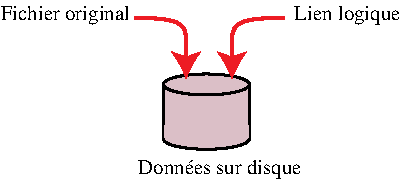
\includegraphics{cmds-unix/log-links}
%\epsfbox{_Images/cmds-unix/symb-links.eps}
\includegraphics{cmds-unix/symb-links}
\caption{\label{fig-cmds-links}Diff{\'e}rence entre les liens symboliques et les
liens logiques}
\end{figure}

\begin{remarque}
Deux ou plusieurs fichiers li{\'e}s par un lien logique doivent r{\'e}sider
sur le m{\^e}me syst{\`e}me de fichiers.
\end{remarque}

%%%%%%%%%%%%%%
\subsubsection{Visualisation du nombre de liens avec la commande {\tt ls}}

\begin{example}
Si l'on prend l'exemple des commandes suivantes~:
\begin{verbatim}
% ls -l
arthur lancelot merlin
% ln -s lancelot dulac
% ln merlin enchanteur
% ls -l
-rw-r--r-- 1 schmoll nobody 37 Jul 25 12:00 arthur
lrw-r--r-- 1 schmoll nobody 37 Jul 25 12:03 dulac -> lancelot
-rwxr-xr-x 2 schmoll nobody 37 Jul 25 12:01 enchanteur
-rw-r--r-- 1 schmoll nobody 37 Jul 25 12:02 lancelot
-rwxr-xr-x 2 schmoll nobody 37 Jul 25 12:01 merlin
\end{verbatim}
donc
\begin{itemize}
	\item {\tt dulac} est un lien symbolique sur {\tt lancelot},
	\item {\tt enchanteur} est un lien logique vers les m{\^e}mes informations
			que celles point{\'e}es par le fichier {\tt merlin}.
\end{itemize}

\index{lien!visualisation du nombre de}On remarque que le fichier {\tt dulac} est de
type <<~{\sl lien}~>> et pointe vers le fichier {\tt lancelot}. Le
nombre de liens pour {\tt dulac} est {\bf 1} (un lien vers lancelot).
\end{example}

\begin{definition}{En conclusion, pour les liens symboliques}
L'information sur le disque est acc{\'e}d{\'e}e uniquement par le fichier
<<~{\tt lancelot}~>>. \\
Lorsqu'on acc{\`e}de au fichier <<~{\tt dulac}~>>, le syst{\`e}me,
renvoie l'identifiant du fichier  <<~{\tt lancelot}~>>. Par
cons{\'e}quent, si le fichier <<~{\tt lancelot}~>> est d{\'e}truit,
<<~{\tt dulac}~>> perdra les r{\'e}f{\'e}rences aux donn{\'e}es.
\end{definition}

\begin{definition}{En conclusion, pour les liens logiques}
Par contre, les types des fichiers <<~{\tt merlin}~>> et <<~{\tt
enchanteur}~>> correspondent {\`a} un <<~{\sl fichier r{\'e}gulier}~>>
ou <<~{\sl standard}~>>. De plus, la commande <<~{\tt ls -l}~>> indique
{\bf deux liens}. En effet, les {\it secteurs} sur le disque physique
correspondent {\`a} deux noms diff{\'e}rents (fichiers {\tt merlin} et
{\tt enchanteur}).

L'information ne r{\'e}side q'une seule fois sur le disque mais elle
peut {\^e}tre acc{\'e}d{\'e}e par deux noms de fichiers diff{\'e}rents.
Par cons{\'e}quent, si le fichier <<~{\tt merlin}~>> est d{\'e}truit,
le syst{\`e}me a toujours acc{\`e}s aux donn{\'e}es via le fichier
<<~{\tt enchanteur}~>>.

\index{lien!logique!recherche des liaisons entre}Le seul moyen de conna{\^i}tre les liaisons entre deux liens logiques est de
conna{\^i}tre l'identifiant sur le disque (<<~\textsl{i-node}~>>) et de
rechercher les fichiers le r{\'e}f{\'e}ren\c{c}ant.
\end{definition}

Le tableau \ref{tab-cmds-equiv-mvcpln} montre les correspondances des commandes
{\tt cp}, {\tt mv} et {\tt ln} entre les syst{\`e}mes d'exploitations {\Unix},
{\OpenVMS} et {\DOS}.

\begin{table}[hbtp]
\centering
\begin{tabular}{|c|c|c|}
	\hline
		{\Unix}		&	{\OpenVMS}	&	{\DOS}					\\
	\hline \hline
		{\tt cp}		&	{\tt COPY}		&	{\tt COPY}				\\
		{\tt mv}		&	{\tt RENAME}	&	{\tt REN}	\\
		{\tt ln}		&	{\tt SET FILE/ENTER} 	&	Pas d'{\'e}quivalence	\\
	\hline
\end{tabular}
\caption{\label{tab-cmds-equiv-mvcpln}\'{E}quivalence des commandes {\tt cp},
{\tt mv} et {\tt ln} entre {\Unix},{\OpenVMS} et {\DOS}}
\end{table}

%%%%%%%%%%%
\subsection{Effacement d'un fichier - Commande {\tt rm}}

\begin{definition}{Syntaxe}
\begin{verbatim}
rm [-irf] fichier...
\end{verbatim}
\end{definition}

\index{rm@\texttt{rm}}La commande <<~{\tt rm}~>> est utilis{\'e}e pour effacer des fichiers. Une
fois effac{\'e}s, les fichiers ne peuvent plus {\^e}tre r{\'e}cup{\'e}r{\'e}s\footnote{{\`a}
moins, biens{\^u}r, de diposer d'un syst{\`e}me de sauvegarde}. La commande {\tt
rm }exige au moins un argument. Si plusieurs arguments sont fournis {\`a} la
commande, tous les fichiers sp{\'e}cifi{\'e}s seront effac{\'e}s en fonction des
modes de protections.

L'option <<~{\tt -r}~>> (r{\'e}cursif) indique la r{\'e}cursivit{\'e} et permet d'effacer un r{\'e}pertoire et tout son contenu.

L'option <<~{\tt -i}~>> (interactive) demande une confirmation (y ou n) sur chaque fichier {\`a} effacer.

L'option <<~{\tt -f}~>> (force) ne fait plus tenir compte {\`a} <<~{\tt rm}~>> des protections du fichier, mais uniquement du
propri{\'e}taire. Vous pouvez donc effacer vos fichiers, m{\^e}me s'ils sont prot{\'e}g{\'e}s.

\begin{center}
{\large
	{\bf
		ATTENTION AUX CATASTROPHES AVEC LES
		OPTIONS <<~{\tt -f}~>> ET SURTOUT <<~{\tt -r}~>> !!!
	}
}
\end{center}

Le tableau \ref{tab-cmds-equiv-rm} donne les correspondances des
diff{\'e}rents comportements de la commande {\tt rm} entre les syst{\`e}mes
d'exploitations {\Unix}, {\OpenVMS} et {\DOS}.

\begin{table}[hbtp]
\centering
\begin{tabular}{|c|c|c|}
	\hline
		{\Unix}			&	{\OpenVMS}		&	{\DOS}					\\
	\hline \hline
		{\tt rm}		&	{\tt DELETE}	&	{\tt DEL}				\\
		{\tt rm -i}		&	{\tt DELETE/CONFIRM}
											&	Pas d'{\'e}quivalence	\\
	\hline
\end{tabular}
\caption{\label{tab-cmds-equiv-rm}\'{E}quivalences de la commande
{\tt rm} entre {\Unix},{\OpenVMS} et {\DOS}.}
\end{table}

%%%%%%%%%%%%%%%%%%%%%%%%%%%%%%%%%%%%%%%%
\section{\label{cmds-protect}Protections sur les fichiers}

%%%%%%%%%%%%
\subsection{\label{cmds-unix-id}Notion d'identit{\'e} sous {\Unix}}

Comme tout syst{\`e}me multi-utilisateurs, multi-t{\^a}ches, vous devez vous
identifer avant de pouvoir travailler sous {\Unix} par~:
\begin{itemize}
	\item	votre nom de login ou {\sl logname},
	\item	votre mot de passe.
\end{itemize}

D{\`e}s que vous {\^e}tes authentifi{\'e}, le syst{\`e}me lance
l'interp{\'e}teur de commande votre num{\'e}ro d'utilisateur~:
l'\index{UID}{\sl UID}\footnote{{\sl UID} = User Identifier}. Il lui
associe aussi un ou plusieurs groupes (en fonction du profil
utilisateur)~: le \index{GID}{\sl GID}\footnote{{\sl GID} = Group Identifier}.

A partir de ce moment, tous les sous-processes g{\'e}n{\'e}r{\'e}s seront lanc{\'e}s
sous la m{\^e}me identit{\'e}, c'est {\`a} dire avec les m{\^e}mes {\sl UID}/{\sl GID}.

\index{fichier!propri{\'e}taire}Chaque fichier sous {\Unix} poss{\`e}de un propri{\'e}taire (associ{\'e} {\`a} un
{\sl UID}) et un groupe (associ{\'e} {\`a} un {\sl GID}). De fa\c{c}on g{\'e}n{\'e}ral, le
propri{\'e}taire et le groupe du fichier correspondent {\`a} ceux du process qui
l'a cr{\'e}{\'e}.

Le propri{\'e}taire du fichier peut en modifier la paternit{\'e}.

Le propri{\'e}taire du fichier peut en modifier le groupe.

Au niveau du m{\'e}canisme des protections, il n'y a pas de liaison entre le
{\sl GID} et l'{\sl UID}. Si un utilisateur a un {\sl UID} donn{\'e}
identique {\`a} celui du fichier et un GID diff{\'e}rent, il se placera au
niveau du propri{\'e}taire. Le num{\'e}ro d'{\sl UID} est unique par
utilisateur.

Il n'y a donc pas de notion de couple ({\sl UID},{\sl GID}) au m{\^e}me
titre que sur {\OpenVMS} avec les UIC <<~{\tt [group,member]}~>>.

L'administrateur du syst{\`e}me ({\tt root} ou {\sl super-user} {\'e}quivalent {\`a}
{\tt SYSTEM} sur {\OpenVMS}) est vu comme le propri{\'e}taire de tous les
fichiers.

Le tableau \ref{tab-cmds-equiv-root} donne les {\'e}quivalences entre {\Unix}
et {\OpenVMS} pour les notions d'identit{\'e}s sur le syst{\`e}me.

\begin{table}[hbtp]
\centering
\begin{tabular}{|c|c|}
	\hline
		{\Unix}			&	{\OpenVMS}				\\
	\hline \hline
		{\tt logname}	&	{\tt Username}			\\
	\hline
		{\tt UID}		&	{\sl UIC}				\\
	\hline
		{\tt GID}		&	groupe dans l'{\sl UIC}	\\
	\hline
\end{tabular}
\caption{\label{tab-cmds-equiv-root}\'{E}quivalences pour les notions d'identit{\'e}s
entre {\Unix} et {\OpenVMS}}
\end{table}

%%%%%%%%%%%%
\subsection{Permissions}

Sous {\Unix}, on distingue trois \index{fichier!modes d'acc{\`e}s}modes
d'acc{\`e}s~:
\begin{itemize}
	\item l'acc{\`e}s en lecture,
	\item l'acc{\`e}s en {\'e}criture,
	\item l'acc{\`e}s en ex{\'e}cution.
\end{itemize}

En fonction du type de fichier (un r{\'e}pertoire ou un fichier standard),
le mode de protection permet de faire les actions d{\'e}crites dans le tableau
\ref{tab-cmds-prot-actions}.

\begin{table}[hbtp]
\centering
\begin{tabular}{|l|p{4cm}|p{4cm}|}
	\hline
		\multicolumn{1}{|c|}{Acc{\`e}s}		&
		Fichier							&
		R{\'e}pertoire						\\
	\hline \hline
		Lecture &
		Le contenu du fichier est visible. &
		le contenu du r{\'e}pertoire est visible\footnote{Visible
		par la commande <<~{\tt ls}~>> par exemple.}.\\
	\hline
		\'{E}criture &
		Le contenu du fichier peut {\^e}tre modifi{\'e}. &
		Le contenu du r{\'e}pertoire peut {\^e}tre
		modifi{\'e}\footnote{Cr{\'e}ation, suppression de fichiers, etc.}. \\
	\hline
		Ex{\'e}cution &
		Le fichier peut {\^e}tre utilis{\'e} en commande\footnote{Reportez vous
		{\`a} la partie \ref{prgm-shell}.}. &
		Le r{\'e}pertoire peut devenir le r{\'e}pertoire courant. \\
	\hline
\end{tabular}
\caption{\label{tab-cmds-prot-actions}Actions possibles en fonction du masque de
protection}
\end{table}

\begin{remarque}
{\bf Remarques sur les protections d'un r{\'e}pertoire}\\
Si le r{\'e}pertoire est accessible en lecture, alors on peut voir les
fichiers qui s'y trouvent par la commande {\tt ls} par exemple.

Si le r{\'e}pertoire est accessible en {\'e}criture, il est alors possible de
faire des manipulations sur les fichiers qui s'y trouvent avec les
commandes {\tt mv}, {\tt cp} et {\tt rm}. Il faut donc bien faire
attention {\`a} ce mode de protection.

Si le r{\'e}pertoire est accessible en ex{\'e}cution, il peut devenir le
r{\'e}pertoire courant avec la commande {\tt cd}.

Par cons{\'e}quent, pour qu'un fichier puisse {\^e}tre effac{\'e}, {\bf il faut avoir les
droits d'{\'e}criture sur le r{\'e}pertoire qui le contient}.
\end{remarque}

Les protections d'un fichier se situent {\`a} trois niveaux~:
\begin{itemize}
	\item le niveau utilisateur ({\tt user}),
	\item le niveau groupe ({\tt group}),
	\item le niveau autre ({\tt other}).
\end{itemize}

La figure \ref{tab-cmds-fileaccess} d{\'e}crit la m{\'e}thode d'acc{\`e}s d'un
processus {\`a} un fichier.

\begin{figure}[hbtp]
\centering
\setlength{\unitlength}{0.92pt}
\begin{picture}(430,283)
	\thinlines
	\put(139,94){\vector(1,0){83}}
	\put(139,171){\vector(1,0){51}}
	\put(139,248){\vector(1,0){51}}
	\put(253,215){\vector(1,0){102}}
	\put(320,172){\vector(1,0){35}}
	\put(320,250){\vector(1,0){33}}
	\put(73,70){\vector(0,-1){29}}
	\put(73,148){\vector(0,-1){29}}
	\put(73,225){\vector(0,-1){29}}
	\put(253,148){\vector(0,-1){38}}
	\put(355,215){\vector(0,-1){102}}
	\put(253,225){\vector(0,-1){10}}
	\put(329,216){Non}	\put(52,131){Non}
	\put(53,210){Non}	\put(329,178){Non}
	\put(51,54){Non}
	\put(329,255){Oui}	\put(155,100){Oui}
	\put(155,176){Oui}	\put(155,253){Oui}
	\put(260,125){Oui}
	\put(10,225){\framebox(128,48){
		\parbox{110pt}{Le fichier a-t-il le m{\^e}me {\sl UID} que le
		processus ?}}}
	\put(191,225){\framebox(128,48){
		\parbox{110pt}{Le masque de protection <<~niveau {\sl Utilisateur}~>>
		autorise-t-il l'acc{\`e}s ?}}}
	\put(10,148){\framebox(128,48){
		\parbox{110pt}{Le masque de protection <<~niveau {\sl Groupe}~>>
		autorise-t-il l'acc{\`e}s ?}}}
	\put(192,148){\framebox(128,60){
		\parbox{110pt}{Le fichier a-t-il un {\sl GID} identique au
		GID ou l'un des groupes secondaire du processus ?}}}
	\put(10,70){\framebox(128,48){
		\parbox{110pt}{Le masque de protection <<~niveau {\sl Autre}~>>
		autorise-t-il l'acc{\`e}s ?}}}
	\put(387,250){\oval(66,32)}
	\put(354,234){\makebox(66,32){Accept{\'e}}}
	\put(354,96){\oval(66,32)}
	\put(321,80){\makebox(66,32){Refus{\'e}}}
	\put(76,26){\oval(66,32)}
	\put(43,10){\makebox(66,32){Refus{\'e}}}
	\put(256,94){\oval(66,32)}
	\put(223,78){\makebox(66,32){Accept{\'e}}}
\end{picture}
\caption{\label{tab-cmds-fileaccess}Algorithme de v{\'e}rification des
droits d'acc{\`e}s sous {\Unix}}
\end{figure}

%%%%%%%%%%%%
\subsection{Changement de protection - Commande {\tt chmod}}

\begin{definition}{Syntaxe}
\begin{verbatim}
chmod mode fichier...
\end{verbatim}
avec~:\\
\begin{tabular}{ll}
		&	{\tt mode}=masque de protections \\
ou bien	&	{\tt mode}=\verb=<u|g|o><+|-><r|w|x>=
\end{tabular}
\end{definition}

Les permissions peuvent {\^e}tre modifi{\'e}es pour un fichier ou un r{\'e}pertoire
par le propri{\'e}taire (ou l'administrateur) en utilisant la commande <<~{\tt
chmod}~>>.

Il est possible de sp{\'e}cifier le nouveau masque de protection de deux fa\c{c}ons~:
\begin{itemize}
	\item pr{\'e}ciser la totalit{\'e} du masque de protection en {\bf octal},
	\item changer le masque de protection niveau par niveau.
\end{itemize}

Le masque de protection en octal s'interpr{\`e}te de la fa\c{c}on suivante~:
\begin{itemize}
	\item le droit de l'acc{\`e}s en lecture correspond {\`a} $2^2 = 4$,
	\item le droit de l'acc{\`e}s en {\'e}criture correspond {\`a} $2^1 = 2$,
	\item le droit de l'acc{\`e}s en ex{\'e}cution correspond {\`a} $2^0 =1$.
\end{itemize}

Le tableau \ref{tab-cmds-prots} r{\'e}sume les diff{\'e}rentes valeurs associ{\'e}es
aux diff{\'e}rents droits d'acc{\`e}s.

\begin{table}[hbtp]
\centering
\begin{tabular}{|l|c|c|c|}
	\hline
	droits d'acc{\`e}s	&
		lecture		&
		{\'e}criture	&
		ex{\'e}cution	\\
					&
		$2^2$		&
		$2^1$		&
		$2^0$		\\
					&
		4			&
		2			&
		1			\\
	\hline
	abr{\'e}viation utilis{\'e}e	&
		{\tt r}		&
		{\tt w}		&
		{\tt x}		\\
	\hline
\end{tabular}
\caption{\label{tab-cmds-prots}Valeurs associ{\'e}es aux diff{\'e}rents droits
d'acc{\`e}s}
\end{table}

Pour affecter les droits d'acc{\`e}s {\`a} un fichier ou un r{\'e}pertoire, il suffit
de proc{\'e}der de la fa\c{c}on suivante~:
\begin{itemize}
	\item on additionne entre elles toutes les autorisations d'acc{\`e}s,
	\item on effectue cette op{\'e}ration pour chaque niveau d'acc{\`e}s
		  ({\sl utilisateur}, {\sl groupe}, {\sl autre}).
\end{itemize}

\begin{example}
Le tableau \ref{tab-cmds-exchmod-oct} donne un exemple de la d{\'e}marche
{\`a} suivre pour affecter prot{\'e}ger un fichier avec un masque en octal.

\begin{table}[hbtp]
\centering
\begin{tabular}{|ccc|ccc|ccc|}
	\hline
		\multicolumn{3}{|c|}{{\sl Utilisateur}}	&
		\multicolumn{3}{|c|}{{\sl Groupe}}		&
		\multicolumn{3}{|c|}{{\sl Autre}}	\\
	\hline
		{\tt r} & {\tt w} & {\tt x}	&
		{\tt r} & {\tt -} & {\tt x}	&
		{\tt -} & {\tt -} & {\tt -}	\\
	\hline
		1              & 1              & 1              &
		1              & 0              & 1              &
		0              & 0              & 0              \\
		$2^2 \times 1$ & $2^1 \times 1$ & $2^0 \times 1$ &
		$2^2 \times 1$ & $2^1 \times 0$ & $2^0 \times 1$ &
		$2^2 \times 0$ & $2^1 \times 0$ & $2^0 \times 0$ \\
		\multicolumn{3}{|c|}{7}	&
		\multicolumn{3}{|c|}{5}		&
		\multicolumn{3}{|c|}{0}	\\
	\hline
\end{tabular}
\caption{\label{tab-cmds-exchmod-oct}Exemple d'affectation d'un masque en octal}
\end{table}
\end{example}

Une autre fa\c{c}on de pr{\'e}ciser le masque de protection est de dire, pour
chaque niveau, quels sont les acc{\`e}s que l'on autorise ou que l'on
interdit par rapport au masque de protection courant. Les abr{\'e}viations
utilis{\'e}es dans ce cas par la commande <<~{\tt chmod}~>> sont d{\'e}crites dans le
tableau \ref{tab-cmds-chmod-relprot}.

\begin{table}[hbtp]
\centering
\begin{tabular}{|c|c|p{4cm}|}
	\hline
	\parbox[c][1cm][c]{4cm}{Abr{\'e}viation utilis{\'e}e par {\tt chmod}}	&
	\parbox[c][1cm][c]{4cm}{Signification pour {\tt chmod}}		&
	\parbox[c][1cm][c]{4cm}{Signification}						\\
	\hline \hline
	{\tt u}	& {\tt user}	&	niveau utilisateur				\\
	{\tt g}	& {\tt group}	&	niveau groupe					\\
	{\tt o}	& {\tt other}	&	niveau autre					\\
	\hline
	{\tt r}	& {\tt read}	&	acc{\`e}s en lecture				\\
	{\tt w}	& {\tt write}	&	acc{\`e}s en {\'e}criture				\\
	{\tt x}	& {\tt execute}	&	acc{\`e}s en ex{\'e}cution				\\
	\hline
\end{tabular}
\caption{\label{tab-cmds-chmod-relprot}Abr{\'e}viations utilis{\'e}es par la
commande <<~{\tt chmod}~>>}
\end{table}

Pour chaque niveau, la commande \index{chmod@\texttt{chmod}}<<~{\tt chmod}~>>
attend un masque de protection du type~:

\begin{center}
\begin{tabular}{ll}
	\verb=<protectionlevel>+<access permisssion>=	&
		pour autoriser un acc{\`e}s,\\
	\verb=<protectionlevel>-<access permisssion>=	&
		pour supprimer un acc{\`e}s.
\end{tabular}
\end{center}

\begin{example}
Les exemples donn{\'e}s dans le tableau \ref{tab-cmds-exchmod-modrel}
montrent comment modifier les protections d'un fichiers par rapport {\`a}
celles qui sont d{\'e}j{\`a}s affect{\'e}es.
\end{example}

\begin{table}[hbtp]
\centering
\begin{tabular}{|c|p{6cm}|}
	\hline
	\multicolumn{1}{|c|}{Exemple}			&
	\multicolumn{1}{|c|}{Signification}		\\
	\hline
	{\tt u+rwx}		&
	Rajoute les droits de lecture, d'{\'e}criture et d'ex{\'e}cution au niveau
	de l'utilisateur.\\
	\hline
	{\tt g+rx}		&
	Rajoute les droits de lecture et d'ex{\'e}cution au niveau du groupe.\\
	{\tt g-w}		&
	Retire les droits en {\'e}criture au niveau du groupe.\\
	\hline
	{\tt o-rwx}		&
	Retire tous les acc{\`e}s pour les autres utilisateurs
	(ni le propri{\'e}taire, ni un utilisateur du m{\^e}me groupe).\\
	\hline
\end{tabular}
\caption{\label{tab-cmds-exchmod-modrel}Exemples de modifications des protections
par rapport {\`a} celles d{\'e}j{\`a} actives}
\end{table}

\begin{remarque}
Il est possible d'avoir des {\'e}quivalences entre les deux fonctionnements. Par
exemple, les deux commandes suivantes sont {\'e}quivalentes~:

\begin{verbatim}
% chmod 750 fichier
% chmod u+rwx g+rx g-w o-rwx fichier
\end{verbatim}
\end{remarque}

%%%%%%%%%%%
\subsection{Remarques sur les protections}

Tous les r{\'e}pertoires inclus dans le chemin d'acc{\`e}s d'un fichier doivent
{\^e}tre accessibles en ex{\'e}cution pour qu'il  puisse {\^e}tre atteind.

Pour prot{\'e}ger un fichier, supprimez le droit d'acc{\`e}s en {\'e}criture sur ce
fichier ainsi que sur le r{\'e}pertoire dans lequel il se trouve.

%%%%%%%%%%%%%%%%%%%%%%%%%%%%%%%%%%%%%%%%
\section{Les filtres}

%%%%%%%%%%%
\subsection{Rappels, Propri{\'e}t{\'e}s}

\noindent {\bf Rappel~:}
\begin{quote}
Un \index{filtre}filtre est une commande devant effectuer une lecture {\`a} partir de
l'entr{\'e}e standard et une {\'e}criture sur la sortie standard. La figure
\ref{fig-cmds-rapp-filter} en montre le fonctionnement.
\end{quote}

\begin{figure}[hbtp]
\centering
%\epsfbox{_Images/cmds-unix/rapp-filter.eps}
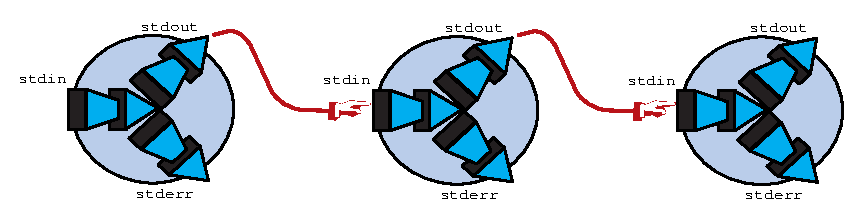
\includegraphics{cmds-unix/rapp-filter}
\caption{\label{fig-cmds-rapp-filter}Rappel sur les filtres}
\end{figure}

\noindent {\bf Propri{\'e}t{\'e}s~:}
\begin{quote}
Par d{\'e}faut, les filtres lisent sur leur entr{\'e}e standard et affichent le
r{\'e}sultat sur leur sortie standard.

Si un fichier est sp{\'e}cifi{\'e} en argument, l'entr{\'e}e standard est redirig{\'e}e
automatiquement sur celui-ci. S'il y en a plusieurs, ils sont mis bout {\`a}
bout et le filtre redirige son entr{\'e}e standard sur le r{\'e}sultat obtenu.
\end{quote}

%%%%%%%%%%%
\subsection{Filtres d{\'e}j{\`a} vus}

La commande \index{cat@\texttt{cat}}<<~{\tt  cat}~>> fonctionne comme un filtre si elle n'a pas
d'arguments. Elle lit sur son entr{\'e}e standard et la r{\'e}affiche sur sa
sortie standard. La figure \ref{fig-cmds-cat} en illustre son fonctionnement.

\begin{figure}[hbtp]
\centering
%\epsfbox{_Images/cmds-unix/cat.eps}
\includegraphics{cmds-unix/cat}
\caption{\label{fig-cmds-cat}Fonctionnement de la commande <<~{\tt cat}~>>}
\end{figure}

\begin{remarque}
La commande \index{more@\texttt{more}}<<~{\tt more}~>> n'est pas un filtre. Elle lit les
informations sur son entr{\'e}e standard ou bien dans les fichiers pass{\'e}s en
argument, et redirige sur l'{\'e}cran. Elle fait appel aux informations que
le syst{\`e}me connait sur le terminal pour conna{\^\i}tre sa taille, son mode
d'{\'e}mulation, etc{...}
\end{remarque}

%%%%%%%%%%%
\subsection{Filtre {\tt sort}}

\begin{definition}{Syntaxe}
\begin{alltt}
sort [-nd] [-tcaract{\`e}re] [+num{\'e}ro-champ>] [-num{\'e}ro-champ]
            [fichier...]
\end{alltt}
\end{definition}

Le filtre \index{sort@\texttt{sort}}<<~{\tt sort}~>> permet de trier les lignes de caract{\`e}res (suite
d'octets d{\'e}limit{\'e}e par le caract{\`e}re \verb=<CR>=) envoy{\'e}es sur l'entr{\'e}e standard
selon un ensemble de crit{\`e}res.

Il est possible de d{\'e}finir un caract{\`e}re s{\'e}parateur de champ afin
d'effectuer des tris sur une zone particuli{\`e}re. Le tri peut se faire~:
\begin{itemize}
	\item soit num{\'e}riquement en sp{\'e}cifiant l'option <<~{\tt -n}~>>,
	\item soit selon l'ordre {\ASCII} standard (mode par d{\'e}faut),
	\item soit selon l'ordre d{\'e}fini dans un dictionnaire avec l'option
		  <<~{\tt -d}~>>.
\end{itemize}

Les champs sont d{\'e}limit{\'e}s par d{\'e}faut par une tabulation ou de fa\c{c}on
explicite par le caract{\`e}re sp{\'e}cifi{\'e} avec l'option -t<caract{\`e}re>.

La commande sort lit sur son entr{\'e}e standard, effectue le tri et affiche
le r{\'e}sultat sur sa sortie standard.

Comme la plupart des filtres, la commande <<~{\tt sort}~>> accepte des
fichiers en arguments. S'ils sont pr{\'e}cis{\'e}s sur la ligne de commande,
<<~{\tt sort}~>> redirige son entr{\'e}e standard sur leur contenu. Il est
{\'e}galement possible de trier sur un champ particulier en utilisant le
symbole <<~{\tt +}~>> suivi du num{\'e}ro du champ.

\begin{remarque}
<<~{\tt sort}~>> num{\'e}rote les champs {\`a} partir de z{\'e}ro.
\end{remarque}

Si la commande est simple {\`a} utiliser pour effectuer des tris simples,
pour des tris plus complexes, plusieurs tentatives sont bien souvent
n{\'e}cessaires avant de trouver la bonne syntaxe. Ne soyez pas frustr{\'e}s~: la
puissance de la commande pallie cet inconv{\'e}nient. Pour plus de
renseignements, consultez le manuel de r{\'e}f{\'e}rence <<~{\tt sort(1)}~>>.

\begin{example}
\begin{verbatim}
% sort -nt: +2 /etc/passwd
% ls -R | sort
\end{verbatim}
\end{example}

%%%%%%%%%%%
\subsection{Filtre {\tt grep}}

\begin{definition}{Syntaxe}
\begin{verbatim}
grep [-inv] expression [fichier...]
\end{verbatim}
\end{definition}

Le filtre \index{grep@\texttt{grep}}<<~{\tt grep}~>> recherche l'expression pr{\'e}cis{\'e}e sur son entr{\'e}e standard et l'affiche sur sa sortie standard. Cette expression ob{\'e}it aux lois des expressions r{\'e}guli{\`e}res {\Unix} (cf. chapitre \ref{reg-exp}). De fa\c{c}on g{\'e}n{\'e}rale, on sp{\'e}cifie une cha{\^\i}ne de caract{\`e}res.

Les options les plus courantes de la commande <<~{\tt grep}~>> sont~:
\begin{itemize}
	\item l'option <<~{\tt -i}~>> indique {\`a} <<~{\tt grep}~>> qu'il ne faut pas
		  tenir compte des majuscules/minuscules,
	\item l'option <<~{\tt -v}~>> indique {\`a} <<~{\tt grep}~>> qu'il faut afficher
		  les lignes ne contenant pas l'expression pr{\'e}cis{\'e}e en argument,
	\item l'option <<~{\tt -n}~>> permet de voir afficher les num{\'e}ros de
		  lignes courantes.
\end{itemize}

Comme la plupart des filtres, la commande <<~{\tt grep}~>> accepte des
fichiers en arguments. S'ils sont pr{\'e}cis{\'e}s sur la ligne de commande,
<<~{\tt grep}~>> redirige son entr{\'e}e standard sur leur contenu.

\begin{example}
\begin{verbatim}
% grep user /etc/passwd
% ls -l | grep rwxrwxrwx
\end{verbatim}
\end{example}

%%%%%%%%%%%%
\subsection{Filtre {\tt wc}}

\begin{definition}{Syntaxe}
\begin{verbatim}
wc [-lwc] [fichier{...}]
\end{verbatim}
\end{definition}

Le filtre \index{wc@\texttt{wc}}<<~{\tt wc}~>> lit sur son entr{\'e}e standard,  compte le nombre
de lignes (enregistrements s{\'e}par{\'e}s par \verb=<CR>=), le nombre de mots
(enregistrements s{\'e}par{\'e}s par \spacekey ou \tabkey), le nombre de
caract{\`e}res et affiche le r{\'e}sultat sur sa sortie standard.

Les options sont~:\\
\begin{tabular}{l@{\hspace{0.5cm}}l}
	{\tt -l}	&	compte le nombre de lignes,\\
	{\tt -w}	&	compte le nombre de mots,\\
	{\tt -c}	&	compte le nombre de caract{\`e}res.
\end{tabular}

L'ordre des options dans la ligne de commande d{\'e}termine l'ordre de
sortie. Comme la plupart des filtres, la commande <<~{\tt wc}~>> accepte
des fichiers en arguments. S'ils sont pr{\'e}cis{\'e}s sur la ligne de commande,
<<~{\tt wc}~>> redirige son entr{\'e}e standard sur leur contenu.

\begin{example}
\begin{verbatim}
% wc -l /etc/passwd
% ls -l | wc -l
\end{verbatim}
\end{example}

%%%%%%%%%%%%
\subsection{Filtre {\tt cut}}

\begin{definition}{Syntaxe}
{\tt cut -c{\it liste} [fichier...]}\\
{\tt cut -f{\it liste} [-d{\it caract{\`e}re}] [-s] [fichier...]}
\end{definition}

Le filtre \index{cut@\texttt{cut}}<<~{\tt cut}~>> a deux modes de fonctionnement~:

\begin{center}
\begin{tabular}{|p{7cm}|l|}
	\hline
		\multicolumn{1}{|c|}{Mode}		&
		\multicolumn{1}{|c|}{Option}	\\
	\hline \hline
		Extraire des colonnes {\`a} partir de l'entr{\'e}e standard.	&
		option <<~{\tt -c}~>>	\\
		Extraire des champs {\`a} partir de l'entr{\'e}e standard.		&
		option <<~{\tt -f}~>> \\
	\hline
\end{tabular}
\end{center}

Dans les deux modes, <<~{\tt liste}~>> est une s{\'e}quence de num{\'e}ros pour
indiquer {\`a} cut quels sont les champs ou les colonnes {\`a} retenir. Il y a
plusieurs formats possibles pour cette liste~:\\
\begin{tabular}{lp{5cm}}
	<<~{\tt {\sl A}-{\sl B}}~>>	&
	champs ou colonnes {\sl A} {\`a} {\sl B} inclus \\
	<<~{\tt {\sl A}-}~>>			&
	du champ ou colonne {\sl A} jusqu'{\`a} la fin de la ligne \\
	<<~{\tt {\sl A},{\sl B}}~>>	&
	champ ou colonnes {\sl A} et {\sl B} \\
	<<~{\tt -{\sl B}}~>>			&
	du d{\'e}but jusqu'au champ ou colonne {\sl B}
\end{tabular}

Toute combinaison des formats pr{\'e}c{\'e}dents est {\'e}galement possible.

\begin{example}
\begin{verbatim}
% cut -f1,4,6-9 /tmp/fictest
\end{verbatim}
extrait du fichier <<~{\tt /tmp/fictest}~>> les champs 1, 4 et de 6 {\`a} 9.
\end{example}

Dans le cas d'un d{\'e}coupage par champ, il existe une option particuli{\`e}re,
<<~{\tt -d}~>>, pour sp{\'e}cifier le caract{\`e}re s{\'e}parateur de champs. Par
d{\'e}faut, ce caract{\`e}re est la tabulation <<~{\tt TAB}~>>. De m{\^e}me,
l'option <<~{\tt -s}~>>, lors d'un d{\'e}coupage par champ, indique {\`a} cut
d'{\'e}carter toutes les lignes qui ne contiennent pas le s{\'e}parateur.

\begin{remarque}
La commande <<~{\tt cut}~>> commence la num{\'e}rotation des champs {\`a} 1 alors
que <<~{\tt sort}~>> commence {\`a} 0. Il y a un moyen facile de s'en rappeler
en notant que sort contient un z{\'e}ro dans son nom (en fait un <<~{\tt
o}~>>) contrairement {\`a} <<~{\tt cut}~>>.
\end{remarque}

Comme la plupart des filtres, la commande <<~{\tt cut}~>> accepte des
fichiers en arguments. S'ils sont pr{\'e}cis{\'e}s sur la ligne de commande,
<<~{\tt cut}~>> redirige son entr{\'e}e standard sur leur contenu.

\begin{example}
\begin{verbatim}
% cut -f3,7 -d: /etc/passwd
% date | cut -c1-3
% ps -ef | cut -c48- | sort
\end{verbatim}
\end{example}
